\documentclass[a4paper,fontsize=12pt]{scrartcl}
\usepackage{tikz}
\begin{document}
\section*{Yuli Zhi}
\subsection*{Weight matrix}
$$ W=\left(\begin{array}{ccccccccccc}
0.0&0.33&-0.33&1.0&0.33&0.33&1.0&-0.33&1.0&0.33&-0.33\\0.33&0.0&-1.0&0.33&1.0&-0.33&0.33&-1.0&0.33&1.0&0.33\\-0.33&-1.0&0.0&-0.33&-1.0&0.33&-0.33&1.0&-0.33&-1.0&-0.33\\1.0&0.33&-0.33&0.0&0.33&0.33&1.0&-0.33&1.0&0.33&-0.33\\0.33&1.0&-1.0&0.33&0.0&-0.33&0.33&-1.0&0.33&1.0&0.33\\0.33&-0.33&0.33&0.33&-0.33&0.0&0.33&0.33&0.33&-0.33&-1.0\\1.0&0.33&-0.33&1.0&0.33&0.33&0.0&-0.33&1.0&0.33&-0.33\\-0.33&-1.0&1.0&-0.33&-1.0&0.33&-0.33&0.0&-0.33&-1.0&-0.33\\1.0&0.33&-0.33&1.0&0.33&0.33&1.0&-0.33&0.0&0.33&-0.33\\0.33&1.0&-1.0&0.33&1.0&-0.33&0.33&-1.0&0.33&0.0&0.33\\-0.33&0.33&-0.33&-0.33&0.33&-1.0&-0.33&-0.33&-0.33&0.33&0.0\\\end{array}\right)$$
\subsection*{Test 1}
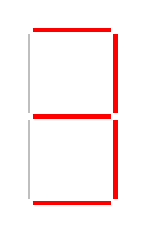
\begin{tikzpicture}
\draw[ultra thick,color=red](0,2.20)--(1,2.20);
\draw[thick,color=lightgray](-.05,1.15)--(-.05,2.15);
\draw[ultra thick,color=red](1.05,1.15)--(1.05,2.15);
\draw[ultra thick,color=red](0,1.10)--(1,1.10);
\draw[thick,color=lightgray](-.05,0.05)--(-.05,1.05);
\draw[ultra thick,color=red](1.05,0.05)--(1.05,1.05);
\draw[ultra thick,color=red](0,0)--(1,0);
\end{tikzpicture}
0
 -4.333 \qquad
 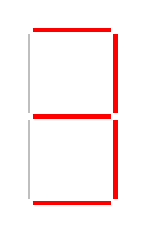
\begin{tikzpicture}
\draw[ultra thick,color=red](0,2.20)--(1,2.20);
\draw[thick,color=lightgray](-.05,1.15)--(-.05,2.15);
\draw[ultra thick,color=red](1.05,1.15)--(1.05,2.15);
\draw[ultra thick,color=red](0,1.10)--(1,1.10);
\draw[thick,color=lightgray](-.05,0.05)--(-.05,1.05);
\draw[ultra thick,color=red](1.05,0.05)--(1.05,1.05);
\draw[ultra thick,color=red](0,0)--(1,0);
\end{tikzpicture}
3
 -16.333 \qquad
 \qquad
 \subsection*{Test 2}
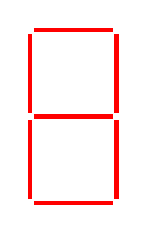
\begin{tikzpicture}
\draw[ultra thick,color=red](0,2.20)--(1,2.20);
\draw[ultra thick,color=red](-.05,1.15)--(-.05,2.15);
\draw[ultra thick,color=red](1.05,1.15)--(1.05,2.15);
\draw[ultra thick,color=red](0,1.10)--(1,1.10);
\draw[ultra thick,color=red](-.05,0.05)--(-.05,1.05);
\draw[ultra thick,color=red](1.05,0.05)--(1.05,1.05);
\draw[ultra thick,color=red](0,0)--(1,0);
\end{tikzpicture}
0
 -0.333 \qquad
 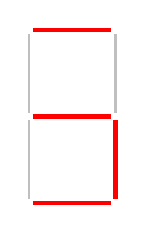
\begin{tikzpicture}
\draw[ultra thick,color=red](0,2.20)--(1,2.20);
\draw[thick,color=lightgray](-.05,1.15)--(-.05,2.15);
\draw[thick,color=lightgray](1.05,1.15)--(1.05,2.15);
\draw[ultra thick,color=red](0,1.10)--(1,1.10);
\draw[thick,color=lightgray](-.05,0.05)--(-.05,1.05);
\draw[ultra thick,color=red](1.05,0.05)--(1.05,1.05);
\draw[ultra thick,color=red](0,0)--(1,0);
\end{tikzpicture}
3
 -9.667 \qquad
 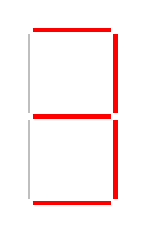
\begin{tikzpicture}
\draw[ultra thick,color=red](0,2.20)--(1,2.20);
\draw[thick,color=lightgray](-.05,1.15)--(-.05,2.15);
\draw[ultra thick,color=red](1.05,1.15)--(1.05,2.15);
\draw[ultra thick,color=red](0,1.10)--(1,1.10);
\draw[thick,color=lightgray](-.05,0.05)--(-.05,1.05);
\draw[ultra thick,color=red](1.05,0.05)--(1.05,1.05);
\draw[ultra thick,color=red](0,0)--(1,0);
\end{tikzpicture}
3
 -16.333 \qquad
 \end{document}